\section{Lampiran}

\subsection{Pernyataan Tidak Melakukan Kecurangan}
\noindent
\fbox{
  \begin{minipage}{\dimexpr\linewidth-2\fboxsep-2\fboxrule\relax}
    \vspace{0.2cm}
    Tugas ini disusun sepenuhnya tanpa bantuan kecerdasan buatan (\textit{Generative AI}), melainkan hasil pemikiran dan analisis mandiri.
    
    \begin{flushright}
      \vspace{0.5cm}
      
\includegraphics[width=3cm]{public/nus.jpeg} \\
      {Stevanus Agustaf Wongso} \\[0.5cm]
      
      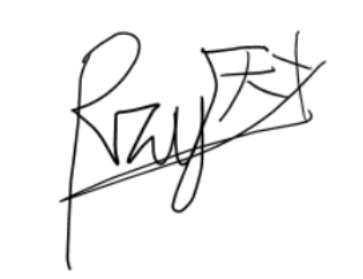
\includegraphics[width=3cm]{public/wen.png} \\
      {Ray Owen Martin} \\[0.5cm]
      
      
\includegraphics[width=3cm]{public/atil.jpeg} \\
      {Athilla Zaidan Zidna Fann} \\[0.5cm]
      \vspace{0.2cm}
    \end{flushright}
  \end{minipage}
}

\subsection{Tautan Repository Github}

Repository Github untuk proyek ini dapat diakses di: \url{https://github.com/AthillaZaidan/Tubes3_Pasti-Gacor-Zeus}

\subsection{Tabel Checklist Spesifikasi}
\begin{table}[H]
    \centering
    \renewcommand{\arraystretch}{1.5} 
    \begin{tabular}{|c|p{10cm}|c|c|}
        \hline
        \textbf{No} & \multicolumn{1}{c|}{\textbf{Poin}} & \textbf{Ya} & \textbf{Tidak} \\
        \hline
        1 & Extension berhasil di-build dan di-load tanpa kesalahan pada chromium browser dan dikembangkan dengan TypeScript & v & \\
        \hline
        2 & KMP dan Boyer-Moore diimplementasikan \textit{from scratch} & v & \\
        \hline
        3 & Regex menghandle format \textless kata\textgreater\textless angka\textgreater\ dan berbagai \textit{edge case} & v & \\
        \hline
        4 & Pencarian KMP \& BM membaca \texttt{keyword.txt} secara iteratif dan tidak menggunakan \textit{built-in search function} atau \textit{library} eksternal & v & \\
        \hline
        5 & \textit{Exact matching} dan \textit{fuzzy matching} berjalan benar & v & \\
        \hline
        6 & Elemen DOM terdeteksi diberi \textit{highlight} dan terhapus saat \textit{rescanning} & v & \\
        \hline
        7 & \textit{Tooltip} muncul saat \textit{hover} dengan informasi \textit{keyword}, algoritma, kemunculan, dan waktu eksekusi & v & \\
        \hline
        8 & \textit{Popup} menampilkan statistik \textit{realtime} (total \textit{keyword}, perbandingan, waktu eksekusi, jumlah \textit{match}) & v & \\
        \hline
        9 & {[Bonus]} Membuat Video & & v \\
        \hline
        10 & {[Bonus]} Implementasi Algoritma Aho-Corasick dan Rabin Karp & v & \\
        \hline
        11 & {[Bonus]} Implementasi \textit{Censorship} / \textit{Blur} Teks & v & \\
        \hline
        12 & {[Bonus]} Implementasi \textit{Optical Character Recognition} pada Gambar & v & \\
        \hline
    \end{tabular}
\end{table}

\subsection{Tabel Pembagian Tugas}
\begin{table}[H]
    \centering
    \renewcommand{\arraystretch}{1.5}
    \begin{tabular}{|p{5cm}|p{8cm}|}
        \hline
        Nama & Bagian \\
        \hline
        Stevanus Agustaf Wongso & Rabin-Karp dan Boyer-Moore, laporan \\
        \hline
        Ray Owen Martin & KMP dan Aho-Corasick, laporan \\
        \hline
        Athilla Zaidan Zidna Fann & RegEx, Weighted Levenshtein, OCR, censorship, laporan \\
        \hline
    \end{tabular}
\end{table}

